% !TEX root = ../main.tex
\chapter{Kinematikk}
\label{Chapter:kinematikk}
\intro{En stor del av fysikken handler om å beskrive og forutsi posisjon og bevegelse for objekter (legemer). Kinematikk er læren om \textit{hvordan}legemer beveger seg. I kinematikken konsentrerer vi oss derfor om begreper som posisjon ($\vec{s}$), hastighet ($\vec{v}$) og akselerasjon ($\vec{a}$), som er verktøyene vi trenger for å beskrive bevegelse. Dette gir det rette grunnlaget for \textit{dynamikken} (/kraftlære), som kommer i neste kapittel, og handler om \textit{årsaken} legemers bevegelse.}

\spm{}{%
\item Hva er sammenhengen mellom posisjon, hastighet og akselerasjon?
\item Hvordan beskriver vi bevegelse med matematikk?
\item Hva er forskjellen på beskriven av bevegelse i 1 dimensjon og flere dimensjoner?}

\section{Hva er kinematikk?}
Kinematikk er studiet av hvordan objekter beveger seg, uten å vurdere (den mekaniske) årsaken til bevegelsen. For å bekrive dette effektivt er det spesielt tre begreper vi er ute etter, med hver sine forkortelser (i parentes):

\[\textrm{strekning ($\vec{s}$)}\quad,\quad\textrm{hastighet ($\vec{v}$)}\quad\textrm{og}\quad\textrm{akselerasjon ($\vec{a}$)}\]

Disse begrepene er alle sammen beskrevet som vektorer (derfor har de piler), ettersom de innbefatter konsepter som har både størrelse og retning. Sammen utgjør de verktøyene vi trenger for å kunne beskrive alt fra enkle scenario, slik som en ball som ruller ned en bakke og til mer kompliserte systemer, som planetenes bevegelse rundt solen. For å beskrive slike sammenhenger effektivt er det viktig å forstå relasjonene mellom strekning, fart og tid.

\section{Strekning ($\vec{s}$) og hastighet ($\vec{v}$)}
Dersom all bevegelse er langs samme, rette linje så kallder vi bevegelsen \textit{rettlinjet}. I dette tilfellet kan vi beskrive strekning og fart som skalarer, altså uten vektornotasjon. Dersom bevegelsen er krum, må vi bruke vektorer. Dette refererer vi til som \textit{krumlinjet} bevegelse. Vi skal se på begge deler. Merk derfor følgende notasjon:
\begin{itemize}
    \item $s$ er strekning, altså størrelsen på \textbf{avstandsvektoren} $\vec{s}$. Vi kommer nok til å bruke begrep som \textit{posisjon} og \textit{forflytning} i tillegg til strekning og avstand. Poenget er at vi må gjøre forsljell på $s$ \textit{uten} vektortegn og \textit{med} vektortegn.
    \item $v$ kalles \textbf{fart} og er størrelsen på \textbf{hastighetsvektoren} $\vec{v}$.
    \item $a$ er størrelsen på akselerasjonsvektoren $\vec{a}$.
\end{itemize}

En bil som kjører på en rett strekning vekk fra en lyktestolpe tilbakelegger større og større strekning (målt fra lyktestolpen). Vi sier gjerne at strekningen er en funksjon av tid, og skriver $s(t)$:

\[s(t)=\textrm{strekning som funksjon av tid}.\]
% \vspace{-3em}
\begin{figure}[H]
    \centering
    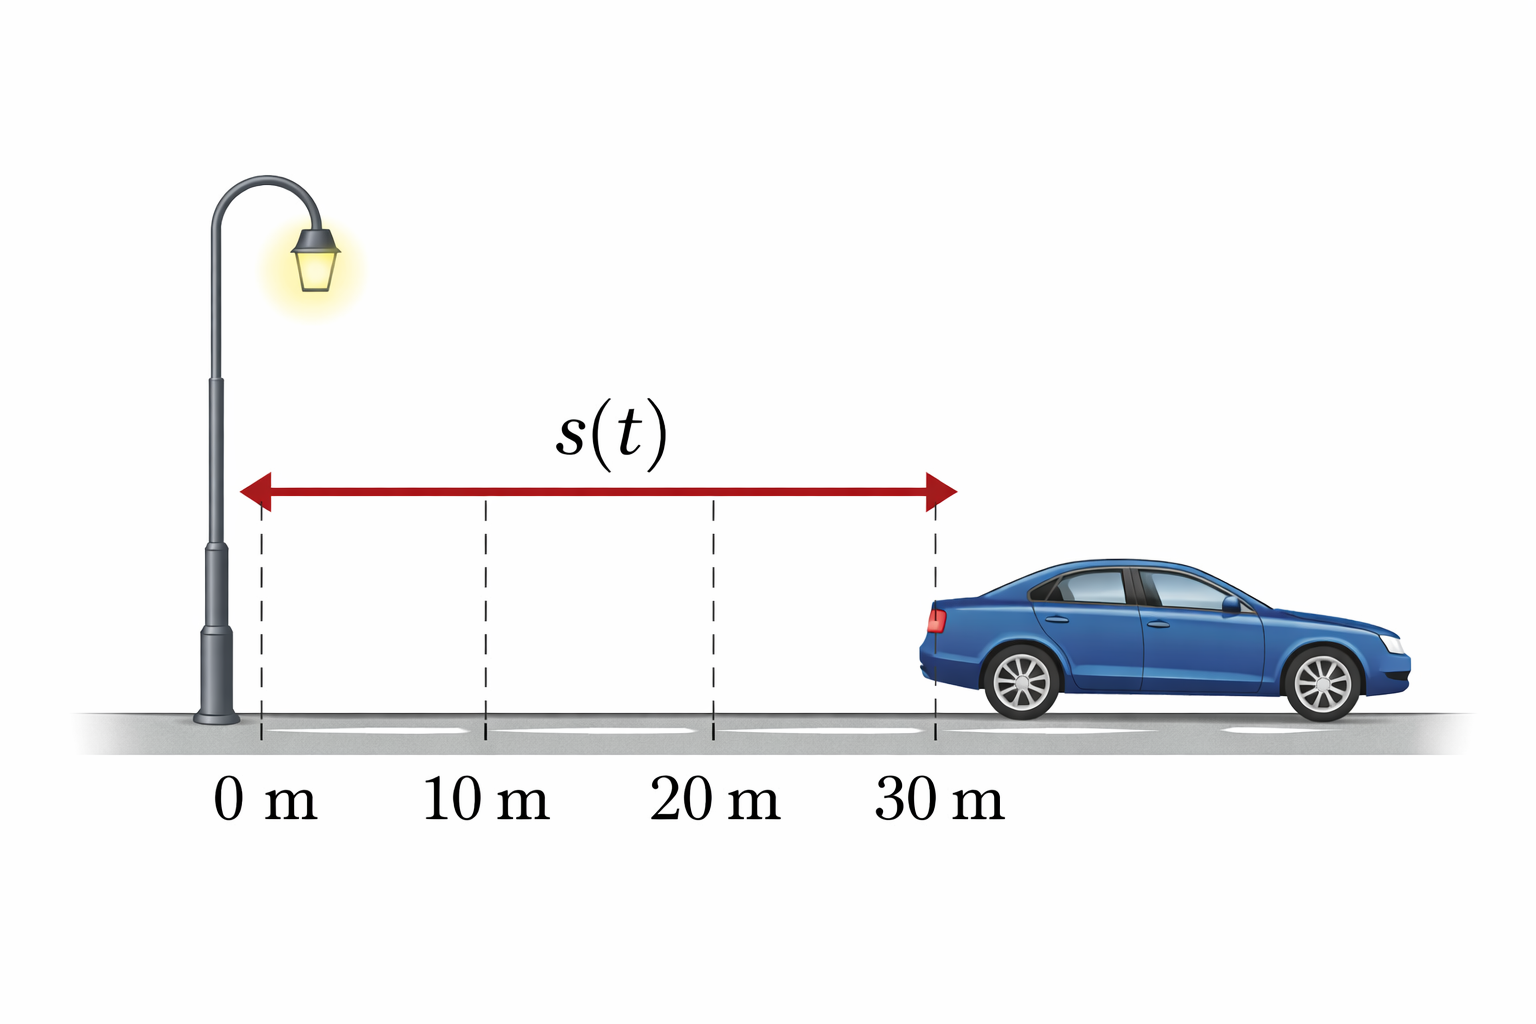
\includegraphics[width=0.7\linewidth, trim={0, 60mm, 0, 60mm},clip]{Images/Kapittel2:Kinematikk/Bil_fra_lyktestolpe.png}
    \caption{Eksempel på avstand mellom en lyktestolpe og forbipasserende bil.}
    \label{fig:fart strekning}
\end{figure}
% \vspace{-3em}
Vi kan illustrere beveglesen til bilen med grafer for fart og strekning. La oss anta at bilen holder konstant fart på $v=36\,\text{km/t}=10\,\text{m/s}$. Da vil strekningen øke med 10 meter hvert sekund, og grafen for strekning vil være en rett linje som stiger jevnt. Grafen for fart vil være en horisontal linje på 10 m/s, siden farten ikke endrer seg. Dette er illustrert i figur \ref{fig:fart- og strekningsgrafer}.
\begin{figure}[H]
\centering
%--- Fartsgraf v(t) ----------------------------------------------------
% Plotområde 4.5 cm × 3.6 cm  |  x: 1.5 cm/s  |  y: 0.3 cm/(m/s), 0–12 m/s
\begin{subfigure}{0.48\textwidth}
  \centering
  \begin{tikzpicture}
    % Lys rutenett
    \foreach \xg in {1.5, 3.0, 4.5}{
      \draw[gray!25, thin] (\xg, 0) -- (\xg, 3.8);
    }
    \foreach \yg in {1.5, 3.0}{
      \draw[gray!25, thin] (0, \yg) -- (4.5, \yg);
    }
    % Akser
    \draw[->, thick] (-0.3, 0) -- (5.1, 0)
          node[right, font=\small] {Tid [s]};
    \draw[->, thick] (0, -0.3) -- (0, 4.4)
          node[above, font=\small] {Fart [m/s]};
    % Tidsaksen: strekmerker
    \foreach \xpos/\xlbl in {0/0, 1.5/1, 3.0/2, 4.5/3}{
      \draw[thin] (\xpos, 2.5pt) -- (\xpos, -2.5pt);
      \node[below=3pt, font=\scriptsize] at (\xpos, 0) {$\xlbl$};
    }
    % Fartsaksen: strekmerker
    \foreach \ypos/\ylbl in {0/0, 1.5/5, 3.0/10}{
      \draw[thin] (-2.5pt, \ypos) -- (2.5pt, \ypos);
      \node[left=4pt, font=\scriptsize] at (0, \ypos) {$\ylbl$};
    }
    % Konstant hastighet v = 10 m/s
    \draw[headCol, thick] (0, 3.0) -- (4.5, 3.0);
    \node[above right=2pt, headCol, font=\scriptsize]
          at (0, 3.0) {$v = 10\ \mathrm{m/s}$};
  \end{tikzpicture}
  \caption{Fartsgraf $v(t)$}
\end{subfigure}\hfill
%--- Posisjonsgraf s(t) ------------------------------------------------
% Plotområde 4.5 cm × 3.6 cm  |  x: 1.5 cm/s  |  y: 1.2 cm per 10 m, 0–30 m
\begin{subfigure}{0.48\textwidth}
  \centering
  \begin{tikzpicture}
    % Lys rutenett
    \foreach \xg in {1.5, 3.0, 4.5}{
      \draw[gray!25, thin] (\xg, 0) -- (\xg, 3.8);
    }
    \foreach \yg in {1.2, 2.4, 3.6}{
      \draw[gray!25, thin] (0, \yg) -- (4.5, \yg);
    }
    % Akser
    \draw[->, thick] (-0.3, 0) -- (5.1, 0)
          node[right, font=\small] {Tid [s]};
    \draw[->, thick] (0, -0.3) -- (0, 4.4)
          node[above, font=\small] {Strekning [m]};
    % Tidsaksen: strekmerker
    \foreach \xpos/\xlbl in {0/0, 1.5/1, 3.0/2, 4.5/3}{
      \draw[thin] (\xpos, 2.5pt) -- (\xpos, -2.5pt);
      \node[below=3pt, font=\scriptsize] at (\xpos, 0) {$\xlbl$};
    }
    % Strekningsaksen: strekmerker
    \foreach \ypos/\ylbl in {0/0, 1.2/10, 2.4/20, 3.6/30}{
      \draw[thin] (-2.5pt, \ypos) -- (2.5pt, \ypos);
      \node[left=4pt, font=\scriptsize] at (0, \ypos) {$\ylbl$};
    }
    % Posisjonslinje s = 10t
    \draw[headCol, thick] (0, 0) -- (4.5, 3.6);
    % Posisjonspunkter fra figur 3.1 (0 m, 10 m, 20 m, 30 m ved t = 0,1,2,3 s)
    \foreach \xpos/\ypos in {0/0, 1.5/1.2, 3.0/2.4, 4.5/3.6}{
      \fill[headCol] (\xpos, \ypos) circle(2.5pt);
    }
    % Kurve-etikett
    \node[above left=2pt, headCol, font=\scriptsize]
          at (2.5, 2.0) {$s = 10t$};
  \end{tikzpicture}
  \caption{Posisjonsgraf $s(t)$}
\end{subfigure}
\caption{Fart- og posisjonsgraf for bil som passerer lyktestolpe med
         konstant hastighet $v = 10\,\mathrm{m/s}$.}
\label{fig:fart- og strekningsgrafer}
\end{figure}

Stigningstallet til strekningsgrafen kan vi regne ut momentant ved derivasjon, eller som gjennomsnittet av endring i posisjon over en periode:
\begin{align*}
    \textrm{v} = \frac{\Delta\textrm{s}}{\Delta\textrm{t}} = \frac{10\textrm{ m}}{1 \textrm{ s}} = 10 \textrm{m/s}
\end{align*}
Som vi kan se ut ifra grafene, er farten det samme som stigningstallet til strekningsgrafen. Fart er altså størrelsen som beskriver endring i posisjon, og uformelt skriver vi gjerne ``trekantformelen'' som mange alt har sett: 

\begin{align}
    v=\frac{s}{t}
\end{align}
\tanke{}{%
Hvordan måler man fart?}
Hvilken strekning er det snakk om i formelen over? Og hvilken tid? Når vi skal måle fart i fysikken, så er det alltid over et visst tidsrom, som vi gjerne kaller $\Delta t$. Det kan jo godt være at farten egentlig endret seg underveis i dette tidsrommet, uten at våre målinger fikk det med seg. Et eksempel kan være om du måler tiden Trine bruker på en 60-meter. La oss si at Trine bruker 12 sekunder. Da er den gjennomsnittlige farten hennes $\bar{v}=60\text{m}/12\text{s}=5\,\text{m}/\text{s}.$ Men det er jo ikke slik å forstå at Trine holdt samme fart hele løpet. I starten var farten gjerne 0m/s, mens den på slutten av løpet kanskje var 10 m/s. Det er derfor viktig å være klar over at når vi snakker om \textit{målt} fart, så handler det alltid om gjennomsnittsfart over et tidsintervall $\Delta t$. Tidsintervallene vi måler på kan være veldig små (slik som i et speedometer), men det er likefullt et gjennomsnitt over dette lille tidsintervallet. For å være litt mer presis definerer vi nå det vi kaller for \textit{gjennomsnittsfart}, som altså er lengden av \textit{gjennomsnittshastighets}-vektoren.

\defn{Gjennomsnittsfart og gjennomsnittshastighet}{
    Matematisk kan gjennomsnittshastigheten uttrykkes som:
    \begin{align}
        \bar{\vec{v}}= \frac{\vec{\Delta s}}{\Delta t}= \frac{s(t+\Delta t) - s(t)}{\Delta t}
    \end{align}
    hvor \( \Delta \vec{s} \) er den totale forflytningen, og \( \Delta t \) er den totale tiden. Lengden av denne vektoren kalles for gjennomsnittsfarten, og er gitt ved:
    \begin{align}
        \bar{v} = |\bar{\vec{v}}| = \frac{|\vec{\Delta s}|}{\Delta t}
    \end{align}
}
Gjennomsnitts\textit{fart}beskriver altså den totale forflytningen til et objekt delt på den totale tiden som har gått. Ettersom forflytning er en vektor, så er gjennomsnitts\textit{hastighet} en vektor. Gjennomsnittsfart er derimot en skalar, siden det er lengden av gjennomsnittshastighetsvektoren. Det er viktig å merke seg at gjennomsnittsfart og gjennomsnittshastighet ikke nødvendigvis er det samme. For eksempel, hvis et objekt beveger seg i en sirkel og returnerer til utgangspunktet, vil den totale forflytningen være null, og dermed vil gjennomsnittshastigheten være null, mens gjennomsnittsfarten vil være positiv, siden den totale tilbakelagte strekningen er omkretsen til sirkelen, og altså større enn null.

\exm{Gjennomsnittsfart i rettlinjet bevegelse}{En bil kjører $60\,\textrm{km}$ på $1.5\,\textrm{t}$. Finn gjennomsnittsfarten i km/t. Gjør om til m/s
}
\svar{%
Vi bruker definisjonen $\bar{v} = \dfrac{\Delta s}{\Delta t}$:
\[\bar{v} = \frac{60\,\textrm{km}}{1{,}5\,\textrm{t}} = \doubleunderline{40\,\textrm{km/t}}\]
Vi bruker omregningsfaktoren $1\,\textrm{km/t} = \frac{1\,000\,\textrm{m}}{3\,600\,\textrm{s}}$:
\[\bar{v} = 40\;\frac{\textrm{km}}{\textrm{t}} \cdot \frac{1\,000\,\textrm{m}}{3\,600\,\textrm{s}} = \frac{40\,000}{3\,600}\,\frac{\textrm{m}}{\textrm{s}} \approx \doubleunderline{11\,\textrm{m/s}}\]
}

\oppgave{Gjennomsnittsfart i rettlinjet bevegelse}{%
En bil kjører $120\,\textrm{km}$ på $1.5\,\textrm{t}$.
\begin{enumerate}[a)]
    \item Finn gjennomsnittsfarten i km/t.
    \item Gjør om til m/s.
    \item En annen bil kjører samme strekning på $90\,\textrm{min}$. Hvem kjørte raskest?
\end{enumerate}
}

\paragraph{Krumlinjet bevegelse.} Når et objekt beveger seg krumlinjet, så blir det hele litt mer komplisert, ettersom den totale forflytningen $\Delta \vec{s}$ ikke nødvendigvis er i samme retning som farten til enhver tid. 

[CHECK HER]


La oss se på et eksempel for å illustrere dette.

\exm{Båt på havet}{To båter skal seile fra punkt $P$ til punkt $R$. Båt 1 seiler i en rett linje fra $P$ til $R$ og bruker 2 timer på seilasen. Båt 2 seiler først 3 km øst til punktet $Q$ og deretter 4 km nord fra $Q$ til $R$. Den bruker 1 time på seilasen øst og 1 time på seilasen nord.\\
\textbf{a)} Skriv ned avstandsvektorene $\vec{\Delta s}_\text{PQ}$, $\vec{\Delta s}_\text{QR}$ og $\vec{\Delta s}_\text{PR}$ som beskriver de relevante forflytningene.\\
\textbf{b)} Hva er gjennomsnittsfarten til båt 1?\\
\textbf{c)} Hva er gjennomsnittsfarten til båt 2 på hver av de to delstrekningene? Hva er den totale gjennomsnittsfarten til båt 2?\\
\textbf{d)} Hva sier disse utregningene om begrepet gjennomsnittsfart?
}

\svar{%
\noindent
\begin{minipage}[t]{0.55\linewidth}
  \vspace{0pt}
  \begin{enumerate}[\textbf{a)}]
    \item Forflytningsvektorene (se figur):
          \[\vec{\Delta s}_{PQ}=[3,\;0]\,\textrm{km},\quad
            \vec{\Delta s}_{QR}=[0,\;4]\,\textrm{km}\]
          \[\vec{\Delta s}_{PR}=[3,\;4]\,\textrm{km}\]
    \item Båt 1 seiler direkte. Forflytningens størrelse:
          \[|\vec{\Delta s}_{PR}|=\sqrt{3^2+4^2}=\doubleunderline{5\,\textrm{km}}\]
          Gjennomsnittsfart (2 timer totalt):
          \[\doubleunderline{\bar{v}_1=\frac{5\,\textrm{km}}{2\,\textrm{t}}=2{,}5\,\textrm{km/t}}\]
    \item Gjennomsnittsfart per etappe for båt 2:
          \[\bar{v}_{PQ}=3\,\textrm{km/t},\quad\bar{v}_{QR}=4\,\textrm{km/t}\]
          Total gjennomsnittsfart for båt 2 (forflytning $=5\,\textrm{km}$, tid $=2\,\textrm{t}$):
          \[\doubleunderline{\bar{v}_2=\frac{5\,\textrm{km}}{2\,\textrm{t}}=2{,}5\,\textrm{km/t}}\]
    \item Selv om båt 2 hadde ulik fart på de to etappene (3 og $4\,\textrm{km/t}$), er den totale gjennomsnittsfarten identisk med båt 1. Gjennomsnittsfart avhenger kun av total forflytning og total tid – ikke av hvordan farten varierte underveis.
  \end{enumerate}
\end{minipage}%
\hfill
\begin{minipage}[t]{0.40\linewidth}
  \vspace{0pt}
  \centering
  \begin{tikzpicture}
    % Kompassindikator
    \draw[->,thin,gray!60](0.2,4.2)--(0.2,4.8)
          node[above,font=\scriptsize]{N};
    \draw[->,thin,gray!60](0.2,4.2)--(0.8,4.2)
          node[right,font=\scriptsize]{Ø};
    % Østlig etappe
    \draw[->,thick,headCol](0,0)--(3,0)
          node[midway,below=4pt,font=\small]{$3\,\textrm{km}$};
    % Nordlig etappe
    \draw[->,thick,defscol](3,0)--(3,4)
          node[midway,right=4pt,font=\small]{$4\,\textrm{km}$};
    % Forflytningsvektor
    \draw[->,very thick,oppsumcol](0,0)--(3,4)
          node[midway,above left=2pt,font=\small]{$\vec{\Delta s}_{PR}=5\,\textrm{km}$};
    % Rett vinkel
    \draw (3,0)++(-0.22,0)--++(0,0.22)--++(0.22,0);
    % Punkter
    \fill(0,0) circle(2pt) node[below left=2pt,font=\small]{$P$};
    \fill(3,0) circle(2pt) node[below right=2pt,font=\small]{$Q$};
    \fill[oppsumcol](3,4) circle(2pt) node[above right=1pt,font=\small]{$R$};
  \end{tikzpicture}
\end{minipage}
}


\exm{Karsten Warholm}{Se for deg at Karsten Warholm løper med konstant fart gjennom en sving. Etter 7 sekunder har han løpt fra inngangen av svingen (punkt $P$) til midten (punkt $Q$). Radiusen i svingen er 36 meter.\\
\textbf{a)} Finn $\Delta s$ mellom punktene $P$ og $Q$. Hvordan kan vi beskrive Karstens posisjon og fart i dette tilfellet?\\
\textbf{b)} Hva er gjennomsnittsfarten på strekningen?}

\svar{%
\noindent
\begin{minipage}[t]{0.55\linewidth}
  \vspace{0pt}
  \begin{enumerate}[\textbf{a)}]
    \item Buelengden fra $P$ til $Q$ (en kvart sirkel):
          \[\Delta s=\tfrac{1}{4}\cdot 2\pi r
            =\tfrac{\pi\cdot 36}{2}=18\pi\approx \doubleunderline{56{,}5\,\textrm{m}}\]
          Forflytningens størrelse (korde $PQ$):
          \[|\vec{\Delta s}|=\sqrt{36^2+36^2}
            =36\sqrt{2}\approx 50{,}9\,\textrm{m}\]
          Merk at farten $|\vec{v}|$ er konstant, men \emph{retningen} endrer seg kontinuerlig (jf.\ pilene i figuren) – hastigheten er derfor \emph{ikke} konstant.
    \item Dersom vi \textit{vet} at Karsten løper i en bue, bruker vi buelengden:
          \[\doubleunderline{\bar{v}=\frac{18\pi\,\textrm{m}}{7\,\textrm{s}}\approx 8{,}1\,\textrm{m/s}}\]
          Dersom vi \textit{ikke vet} det og kun kjenner posisjonene $P$ og $Q$, bruker vi korden:
          \[\bar{v}=\frac{36\sqrt{2}\,\textrm{m}}{7\,\textrm{s}}\approx 7{,}3\,\textrm{m/s}\]
          Gjennomsnittsfarten avhenger altså av hvilken informasjon vi har om banen.
  \end{enumerate}
\end{minipage}%
\hfill
\begin{minipage}[t]{0.40\linewidth}
  \vspace{0pt}
  \centering
  \begin{tikzpicture}[scale=0.9]
    % Bane: kvartssirkel fra P=(2.5,0) til Q=(0,2.5)
    \draw[headCol,thick](2.5,0) arc(0:90:2.5);
    % Stiplede radier
    \draw[dashed,gray!60](0,0)--(2.5,0)
          node[midway,below=3pt,font=\scriptsize]{$r{=}36\,\textrm{m}$};
    \draw[dashed,gray!60](0,0)--(0,2.5);
    % Rett vinkel ved sentrum
    \draw(0.22,0)--++(0,0.22)--++(-0.22,0);
    % Forflytningsvektor (korde P til Q)
    \draw[->,very thick,oppsumcol](2.5,0)--(0,2.5)
          node[midway,right=4pt,font=\small]{$\vec{\Delta s}$};
    % Hastighetspiler (tangenter til banen)
    \draw[->,thick,defscol](2.5,0)--(2.5,0.85)
          node[right,font=\scriptsize]{$\vec{v}_P$};
    \draw[->,thick,defscol](0,2.5)--(-0.85,2.5)
          node[above,font=\scriptsize]{$\vec{v}_Q$};
    % Punkter og etiketter
    \fill[headCol](2.5,0) circle(2pt)
          node[below right=1pt,font=\small]{$P$};
    \fill[headCol](0,2.5) circle(2pt)
          node[above left=1pt,font=\small]{$Q$};
    \fill(0,0) circle(1.5pt);
  \end{tikzpicture}
\end{minipage}
}
La oss se på et eksempel der vi vet retningen til en hastighetsvektor og skal finne komponentene.
\exm{Dekomponering av hastighet}{En fugl flyr med fart $v = 15\,\textrm{m/s}$ i en retning som utgjør $\theta = 37°$ over horisontalplanet ($\cos 37° \approx 0{,}80$, $\sin 37° \approx 0{,}60$).\\
\textbf{a)} Finn den horisontale komponenten $v_x$ og den vertikale komponenten $v_y$ av hastigheten.\\
\textbf{b)} Verifiser at $|\vec{v}| = \sqrt{v_x^2 + v_y^2} = 15\,\textrm{m/s}$.}

\svar{%
\noindent
\begin{minipage}[t]{0.55\linewidth}
  \vspace{0pt}
  \begin{enumerate}[\textbf{a)}]
    \item Vi dekomponerer langs de to aksene (se figur):
          \[v_x = v\cos\theta = 15\cdot 0{,}80 = \doubleunderline{12\,\textrm{m/s}}\]
          \[v_y = v\sin\theta = 15\cdot 0{,}60 = \doubleunderline{9\,\textrm{m/s}}\]
    \item Pythagoras bekrefter:
          \[\sqrt{v_x^2+v_y^2}=\sqrt{12^2+9^2}=\sqrt{144+81}=\sqrt{225}=\doubleunderline{15\,\textrm{m/s}}\;\checkmark\]
  \end{enumerate}
  Merk at dette er det samme $9$-$12$-$15$-trekantforholdet (skalert $3$-$4$-$5$) som dukket opp i eksempel 3.2, men nå brukt til å gå fra totalfart til komponenter.
\end{minipage}%
\hfill
\begin{minipage}[t]{0.40\linewidth}
  \vspace{0pt}
  \centering
  % Vektortrekant: v=15, vx=12, vy=9, theta=37°
  \begin{tikzpicture}[font=\small, scale=0.85]
    % Fylt trekant
    \fill[headCol!12](0,0)--(4,0)--(4,3)--cycle;
    % Horisontal komponent vx
    \draw[->,thick,defscol](0,0)--(4,0)
          node[midway,below=3pt]{$v_x=12\,\textrm{m/s}$};
    % Vertikal komponent vy
    \draw[->,thick,oppsumcol](4,0)--(4,3)
          node[midway,right=3pt]{$v_y=9\,\textrm{m/s}$};
    % Totalvektoren v
    \draw[->,very thick,headCol](0,0)--(4,3)
          node[midway,above left=2pt]{$v=15\,\textrm{m/s}$};
    % Rett vinkel
    \draw(4,0)++(-0.28,0)--++(0,0.28)--++(0.28,0);
    % Vinkel theta
    \draw[thin](0.85,0) arc(0:36.87:0.85);
    \node[right=2pt,font=\scriptsize]at(0.80,0.22){$\theta$};
    % Origo
    \fill(0,0) circle(1.5pt);
  \end{tikzpicture}
\end{minipage}
}

\subsubsection{Momentanfart}
Fra eksemplet med de to båtene, samt Karsten Warholm, så ser vi at hva gjennomsnittsfarten beregner til å være, er veldig avhengig av hvor ofte vi måler. Desto kortere tidsintervall vi måler på, desto mer nøyaktig blir resultatet. I praksis kan vi ofte måle posisjonen til et legeme veldig ofte, og dermed kan vi finne ut hva farten er på et gitt tidspunkt. Dette kaller vi for \textit{momentanhastighet}. 

Momentanhastighet er hastigheten til et objekt på et spesifikt tidspunkt. Det beskriver hvor raskt et objekt beveger seg i akkurat det øyeblikket, og er derfor den ``øyeblikkelige'' hastigheten.

Geometrisk kan vi forstå dette ved å betrakte posisjonskurven $s(t)$: gjennomsnittsfarten over intervallet $[t_0,\,t_0+\Delta t]$ er stigningstallet til \textit{sekantlinjen} gjennom punktene $(t_0,\,s(t_0))$ og $(t_0+\Delta t,\,s(t_0+\Delta t))$. Lar vi $\Delta t \to 0$, vil sekantlinjen nærme seg \textit{tangentlinjen} ved $t_0$ (se figuren under). Stigningstallet til tangentlinjen er nettopp den deriverte, og vi skriver:
\[
  v(t_0)
  = \lim_{\Delta t \to 0} \frac{\Delta s}{\Delta t}
  = \frac{ds}{dt}\bigg|_{t=t_0}
\]

%--- Illustrasjon: sekantlinje → tangentlinje når Δt → 0 ---------------
% Kurve: s(t) = 0.2 t²
% P ved t₀=2.0  →  s=0.8,  tangentslope = 0.80
% Q ved t =4.5  →  s=4.05, sekant PQ slope = 1.30  (stiplet)
% R ved t =3.2  →  s=2.048, sekant PR slope = 1.04  (hel)
% Linjeetiketter: «sekant PQ» over PQ ved x=3.8;
%                 «sekant PR» under PR ved x=3.8;
%                 «tangentlinje» under tangent ved x=4.5.
% «Δt→0»: label øverst ved x=3.6, pil ned-venstre til (2.8, 2.6).
\begin{center}
\begin{tikzpicture}[font=\small]
  %--- Akser ---
  \draw[->, thick] (-0.3, 0) -- (5.7, 0) node[right] {$t$};
  \draw[->, thick] (0, -0.3) -- (0, 4.8) node[above] {$s(t)$};
  %--- Posisjonskurve: s = 0.2t² ---
  \draw[headCol, thick, domain=0:4.65, samples=80]
    plot (\x, {0.2*\x*\x});
  %--- Fastpunkt P ---
  \fill[headCol] (2.0, 0.8) circle(2.5pt);
  \node[left=3pt] at (2.0, 0.8) {$P$};
  %--- Sekantlinje PQ (stor Δt) – stiplet, mørkere ---
  \draw[black!55, semithick, dashed]
    (1.4, {1.30*1.4-1.80}) -- (4.7, {1.30*4.7-1.80});
  \fill[black!55] (4.5, 4.05) circle(2pt);
  \node[above left=2pt, black!60, font=\scriptsize] at (4.5, 4.05) {$Q$};
  %--- Sekantlinje PR (liten Δt) – hel linje, lysere ---
  \draw[black!30, semithick]
    (1.3, {1.04*1.3-1.28}) -- (4.8, {1.04*4.8-1.28});
  \fill[black!36] (3.2, 2.048) circle(2pt);
  \node[right=3pt, black!42, font=\scriptsize] at (3.2, 2.048) {$R$};
  %--- Tangentlinje ved P – oransje, tykk ---
  \draw[oppsumcol, thick]
    (1.1, {0.8*1.1-0.8}) -- (4.9, {0.8*4.9-0.8});
  %--- Δt/Δs-trekant (prikket, svak) ---
  \draw[dotted, gray!65, thin] (2.0, 0.8) -- (4.5, 0.8)
        node[midway, below=2pt, gray!80, font=\scriptsize] {$\Delta t$};
  \draw[dotted, gray!65, thin] (4.5, 0.8) -- (4.5, 4.05)
        node[midway, right=2pt, gray!80, font=\scriptsize] {$\Delta s$};
  %--- t-akse-etiketter ---
  \draw[thin] (2.0, 2.5pt) -- (2.0, -2.5pt);
  \node[below=2pt, font=\scriptsize] at (2.0, 0) {$t_0$};
  \draw[thin] (4.5, 2.5pt) -- (4.5, -2.5pt);
  \node[below=2pt, font=\scriptsize] at (4.5, 0) {$t_0{+}\Delta t$};
  %--- Linjeetiketter spredt for å unngå overlapp ---
  % «sekant PQ»: OVER PQ-linjen ved x=3.8 (PQ=3.14, over kurven=2.89)
  \node[above=2pt, black!60, font=\scriptsize]
        at (3.8, {1.30*3.8-1.80}) {sekant $PQ$};
  % «sekant PR»: UNDER PR-linjen ved x=3.8 (PR=2.67, tangent=2.24 nedenfor)
  \node[below=2pt, black!42, font=\scriptsize]
        at (3.8, {1.04*3.8-1.28}) {sekant $PR$};
  % «tangentlinje»: under tangentlinjen, høyre side
  \node[below right=1pt, oppsumcol, font=\scriptsize]
        at (4.5, {0.8*4.5-0.8}) {tangentlinje};
  %--- Δt→0: label øverst, pil kurver ned-venstre til klart rom ---
  \draw[->, thin, black!45]
        (3.6, 4.5) to[out=245, in=85] (2.8, 2.6);
  \node[right=1pt, black!50, font=\scriptsize] at (3.6, 4.5)
        {$\Delta t \to 0$};
\end{tikzpicture}
\end{center}

\defn{Momentanhastighet}{
    Matematisk kan momentanfart finnes ved å ta den deriverte av posisjonen med hensyn til tid:
    \begin{align}
        \vec{v} &= \frac{d\vec{s}}{dt}
    \end{align}
    Dette gir oss hastigheten nøyaktig i det øyeblikket vi er interessert i.
}

\exm{Speedometer}{
Tenk deg at du kjører bil og ser på speedometeret. Hastigheten som vises på speedometeret er momentanhastigheten din. Den kan endre seg fra ett sekund til et annet hvis du akselererer eller bremser. \\

\textit{Metode:}
Momentanhastighet er hastigheten til et objekt på et spesifikt tidspunkt. I dette tilfellet viser speedometeret bilens hastighet i sanntid, som kan variere hvis du akselererer eller bremser. Speedometeret gir dermed en direkte måling av bilens momentanhastighet, som er et uttrykk for hvor raskt bilen beveger seg i akkurat det øyeblikket.
}

Den store forskjellen mellom momentanfart og gjennomsnittsfart er at momentanfart ser på hastigheten i et spesifikt øyeblikk, mens gjennomsnittsfart ser på den totale bevegelsen over tid. Momentanfarten kan variere kraftig under en bevegelse, mens gjennomsnittsfarten gir en enkel verdi som representerer hele perioden.

\exm{Momentanhastighet}{Posisjonen til en firhjuling på et jorde er gitt ved $vec{s}(t) = (2t^2, 3t)$ i meter og sekunder.\\
\textbf{a)} Vis at uttrykket for momentanhastigheten $\vec{v}(t)$ til firhjulingen er gitt ved $\vec{v}(t) = (4t, 3)$.\\
\textbf{b)} Hva er momentanhastigheten ved $t = 2\,\textrm{s}$?\\
\textbf{c)} Ved hvilken tid er momentanhastigheten $\vec{v} = (16, 12)\,\textrm{m/s}$?

}

\oppgave{Momentanhastighet}{%
Et legeme beveger seg etter posisjonslikningen $s(t) = 3t^2 + 2t$ (i meter og sekunder).
\begin{enumerate}[a)]
    \item For den som kan derivere: Vis at momentanfarten er gitt ved $v(t) = 6t + 2$.
    \item Hva er momentanhastigheten ved $t = 2\,\textrm{s}$?
    \item Ved hvilken tid er momentanfarten $v = 20\,\textrm{m/s}$?
\end{enumerate}
}

\svar{%
\begin{enumerate}[a)]
  \item Vi deriverer $s(t) = 3t^2 + 2t$ ledd for ledd med potensregelen
    $\frac{d}{dt}(t^n) = nt^{n-1}$:
    \[
      v(t) = \frac{ds}{dt} = 3 \cdot 2t^{2-1} + 2 \cdot 1 = 6t + 2\;\textrm{m/s}
      \quad\checkmark
    \]
  \item Vi setter inn $t = 2\,\textrm{s}$:
    \[
      v(2) = 6 \cdot 2 + 2 = 12 + 2 = \doubleunderline{14\,\textrm{m/s}}
    \]
  \item Vi løser likningen $v(t) = 20\,\textrm{m/s}$:
    \[
      6t + 2 = 20
      \implies 6t = 18
      \implies \doubleunderline{t = 3\,\textrm{s}}
    \]
\end{enumerate}
}


\subsubsection{Konstant fart}
 Vi kan tilslutt merke oss at desom farten ikke endrer seg, men er konstant, da er \textit{momentanfarten} til enhver tid den samme som \textit{gjennomsnittsfarten}. Ved konstant hastighet vil den tilbakelagte distansen være proporsjonal med tiden som har gått.


\oppgave{Konstant hastighet}{%
En syklist kjører med konstant hastighet $v = 8\,\textrm{m/s}$.
\begin{enumerate}[a)]
    \item Hvor langt har syklisten kjørt etter $t = 10\,\textrm{s}$?
    \item Hvor langt har syklisten kjørt etter $t = 2\,\textrm{min}$?
    \item Hvor lang tid tar det å tilbakelegge $s = 2.0\,\textrm{km}$?
\end{enumerate}
}

\oppgave{En oppgave til}{%
Noe om dekomponering av fart i to dimensjoner.
}




\section{Akselerasjon}
Vi har så langt sett at endringen i strekning kalles fart. Men hva kalles endring i fart? Jo, det kalles \textit{akselerasjon}. Eller mer presist, så er akselerasjon et mål på endring i hastighet. Og hastighet har både størrelse og retning (er en vektor). Derfor handler akselerasjon om endring både av fartens størrelse og retning. Hvis akselerasjonen er positiv, øker objektets hastighet, mens en negativ akselerasjon (ofte kalt retardasjon, deselerasjon eller bare bremsing) betyr at hastigheten minker.
\tanke{}{%
Hva tenker du om størrelse og retning på akselerasjonen i følgende to tilfeller?\\
(I) En racerbil kjører med konstant fart på et rett strekke.\\
(II) En racerbil kjører med konstant fart gjennom en sving.
}



%--- Figur 3.3 og 3.4 side om side: konstant vs. varierende akselerasjon ----
% Figur 3.3: s₀=0, v₀=−2 m/s, a=1 m/s² (konstant)
%   s(t)=½t²−2t, v(t)=t−2, a(t)=1
% Figur 3.4: s₀=0, v₀=−2 m/s; a₁=2 m/s² for t∈[0,2 s], a₂=−1 m/s² for t∈[2,5 s]
%   Fase 1: v(t)=2t−2, s(t)=t²−2t
%   Fase 2: v(t)=4−t,  s(t)=2(t−2)−½(t−2)²
%   Kontrollpunkter: s(1)=−1, s(2)=0, s(4)=2(max), s(5)=1.5
%                    v(0)=−2, v(1)=0, v(2)=2, v(4)=0, v(5)=−1
% Skala (begge): x: 0.9 cm/s | y_s: 0.72 cm/m | y_v: 0.6 cm/(m/s) | y_a: 0.6 cm/(m/s²)
\begin{figure}[ht!]
\centering

%=== VENSTRE: Figur 3.3 – konstant akselerasjon ==========================
\begin{minipage}[t]{0.46\textwidth}
\centering

%--- Posisjonsgraf s(t) = ½t² − 2t ---
\begin{tikzpicture}
  \foreach \xg in {0.9, 1.8, 2.7, 3.6, 4.5}{
    \draw[gray!25, thin] (\xg, -1.6) -- (\xg, 2.0); }
  \foreach \yg in {-1.44, -0.72, 0.72, 1.44}{
    \draw[gray!25, thin] (0, \yg) -- (4.5, \yg); }
  \draw[->, thick] (-0.3, 0) -- (5.2, 0)
        node[right, font=\small] {$t$ [s]};
  \draw[->, thick] (0, -1.8) -- (0, 2.2)
        node[above, font=\small] {Posisjon [m]};
  \foreach \xpos/\xlbl in {0.9/1, 1.8/2, 2.7/3, 3.6/4, 4.5/5}{
    \draw[thin] (\xpos, 2.5pt) -- (\xpos, -2.5pt);
    \node[below=3pt, font=\scriptsize] at (\xpos, 0) {$\xlbl$}; }
  \foreach \ypos/\ylbl in {-1.44/{-2}, -0.72/{-1}, 0.72/1, 1.44/2}{
    \draw[thin] (-2.5pt, \ypos) -- (2.5pt, \ypos);
    \node[left=4pt, font=\scriptsize] at (0, \ypos) {$\ylbl$}; }
  \node[below left=1pt, font=\scriptsize] at (0, 0) {$0$};
  \draw[headCol, thick, domain=0:4.5, samples=60]
    plot (\x, {(4/9)*\x*\x - 1.6*\x});
  \node[above right=2pt, headCol, font=\scriptsize] at (3.6, 1.2) {$s(t)$};
\end{tikzpicture}

\smallskip

%--- Fartsgraf v(t) = t − 2 ---
\begin{tikzpicture}
  \foreach \xg in {0.9, 1.8, 2.7, 3.6, 4.5}{
    \draw[gray!25, thin] (\xg, -1.3) -- (\xg, 2.0); }
  \foreach \yg in {-1.2, -0.6, 0.6, 1.2, 1.8}{
    \draw[gray!25, thin] (0, \yg) -- (4.5, \yg); }
  \draw[->, thick] (-0.3, 0) -- (5.2, 0)
        node[right, font=\small] {$t$ [s]};
  \draw[->, thick] (0, -1.5) -- (0, 2.2)
        node[above, font=\small] {Fart [m/s]};
  \foreach \xpos/\xlbl in {0.9/1, 1.8/2, 2.7/3, 3.6/4, 4.5/5}{
    \draw[thin] (\xpos, 2.5pt) -- (\xpos, -2.5pt);
    \node[below=3pt, font=\scriptsize] at (\xpos, 0) {$\xlbl$}; }
  \foreach \ypos/\ylbl in {-1.2/{-2}, -0.6/{-1}, 0.6/1, 1.2/2, 1.8/3}{
    \draw[thin] (-2.5pt, \ypos) -- (2.5pt, \ypos);
    \node[left=4pt, font=\scriptsize] at (0, \ypos) {$\ylbl$}; }
  \node[below left=1pt, font=\scriptsize] at (0, 0) {$0$};
  \draw[headCol, thick] (0, -1.2) -- (4.5, 1.8);
  \node[above right=2pt, headCol, font=\scriptsize] at (3.5, 1.5) {$v(t)$};
\end{tikzpicture}

\smallskip

%--- Akselerasjonsgraf a(t) = 1 m/s² ---
\begin{tikzpicture}
  \foreach \xg in {0.9, 1.8, 2.7, 3.6, 4.5}{
    \draw[gray!25, thin] (\xg, 0) -- (\xg, 2.2); }
  \draw[gray!25, thin] (0, 1.2) -- (4.5, 1.2);
  \draw[->, thick] (-0.3, 0) -- (5.2, 0)
        node[right, font=\small] {$t$ [s]};
  \draw[->, thick] (0, -0.3) -- (0, 2.6)
        node[above, font=\small] {Akselerasjon [m/s\textsuperscript{2}]};
  \foreach \xpos/\xlbl in {0.9/1, 1.8/2, 2.7/3, 3.6/4, 4.5/5}{
    \draw[thin] (\xpos, 2.5pt) -- (\xpos, -2.5pt);
    \node[below=3pt, font=\scriptsize] at (\xpos, 0) {$\xlbl$}; }
  \foreach \ypos/\ylbl in {0/0, 1.2/1}{
    \draw[thin] (-2.5pt, \ypos) -- (2.5pt, \ypos);
    \node[left=4pt, font=\scriptsize] at (0, \ypos) {$\ylbl$}; }
  \draw[headCol, thick] (0, 1.2) -- (4.5, 1.2);
  \node[above right=2pt, headCol, font=\scriptsize]
        at (0, 1.2) {$a = 1\ \mathrm{m/s}^2$};
  \node[left=4pt, font=\scriptsize, opacity=0] at (0, 0) {$-2$};
\end{tikzpicture}

\caption{Posisjon, fart og akselerasjon ved \emph{konstant} akselerasjon
         ($s_0=0$, $v_0=-2\,\mathrm{m/s}$, $a=1\,\mathrm{m/s}^2$).}
\label{Konstant akselerasjon}
\end{minipage}%
%=== SKILLELINJE ==========================================================
\hspace{4pt}{\color{black!25}\rule[-10cm]{0.4pt}{10cm}}\hspace{4pt}%
%=== HØYRE: Figur 3.4 – varierende akselerasjon ===========================
% Fase 1 (0≤t≤2): a=2 → v=2t−2, s=t²−2t
%   TikZ s: y=(8/9)x²−1.6x  [verifisert: t=1→y=−0.72, t=2→y=0]
% Fase 2 (2≤t≤5): a=−1 → v=4−t, s=2(t−2)−½(t−2)²
%   TikZ s: y=1.6(x−1.8)−(4/9)(x−1.8)²  [verifisert: t=4→y=1.44, t=5→y=1.08]
\begin{minipage}[t]{0.46\textwidth}
\centering

%--- Posisjonsgraf – stykkvis parabolsk ---
\begin{tikzpicture}
  \foreach \xg in {0.9, 1.8, 2.7, 3.6, 4.5}{
    \draw[gray!25, thin] (\xg, -1.6) -- (\xg, 2.0); }
  \foreach \yg in {-0.72, 0.72, 1.44}{
    \draw[gray!25, thin] (0, \yg) -- (4.5, \yg); }
  % Faseskille
  \draw[gray!40, dashed, thin] (1.8, -1.6) -- (1.8, 2.0);
  \draw[->, thick] (-0.3, 0) -- (5.2, 0)
        node[right, font=\small] {$t$ [s]};
  \draw[->, thick] (0, -1.8) -- (0, 2.2)
        node[above, font=\small] {Posisjon [m]};
  \foreach \xpos/\xlbl in {0.9/1, 1.8/2, 2.7/3, 3.6/4, 4.5/5}{
    \draw[thin] (\xpos, 2.5pt) -- (\xpos, -2.5pt);
    \node[below=3pt, font=\scriptsize] at (\xpos, 0) {$\xlbl$}; }
  \foreach \ypos/\ylbl in {-0.72/{-1}, 0.72/1, 1.44/2}{
    \draw[thin] (-2.5pt, \ypos) -- (2.5pt, \ypos);
    \node[left=4pt, font=\scriptsize] at (0, \ypos) {$\ylbl$}; }
  \node[below left=1pt, font=\scriptsize] at (0, 0) {$0$};
  % Fase 1: s=t²−2t → y=(8/9)x²−1.6x
  \draw[headCol, thick, domain=0:1.8, samples=30]
    plot (\x, {(8/9)*\x*\x - 1.6*\x});
  % Fase 2: s=2(t−2)−½(t−2)² → y=1.6(x−1.8)−(4/9)(x−1.8)²
  \draw[headCol, thick, domain=1.8:4.5, samples=30]
    plot (\x, {1.6*(\x-1.8) - (4/9)*(\x-1.8)*(\x-1.8)});
  \node[above right=2pt, headCol, font=\scriptsize] at (3.2, 1.44) {$s(t)$};
  % Usynlig node for lik venstre margin som fig 3.3
  \node[left=4pt, font=\scriptsize, opacity=0] at (0, -1.44) {$-2$};
\end{tikzpicture}

\smallskip

%--- Fartsgraf – stykkvis lineær ---
% Fase 1: v=2t−2 → linje (0,−1.2)→(1.8,1.2)
% Fase 2: v=4−t  → linje (1.8,1.2)→(4.5,−0.6)
\begin{tikzpicture}
  \foreach \xg in {0.9, 1.8, 2.7, 3.6, 4.5}{
    \draw[gray!25, thin] (\xg, -1.3) -- (\xg, 2.0); }
  \foreach \yg in {-1.2, -0.6, 0.6, 1.2}{
    \draw[gray!25, thin] (0, \yg) -- (4.5, \yg); }
  % Faseskille
  \draw[gray!40, dashed, thin] (1.8, -1.5) -- (1.8, 2.2);
  \draw[->, thick] (-0.3, 0) -- (5.2, 0)
        node[right, font=\small] {$t$ [s]};
  \draw[->, thick] (0, -1.5) -- (0, 2.2)
        node[above, font=\small] {Fart [m/s]};
  \foreach \xpos/\xlbl in {0.9/1, 1.8/2, 2.7/3, 3.6/4, 4.5/5}{
    \draw[thin] (\xpos, 2.5pt) -- (\xpos, -2.5pt);
    \node[below=3pt, font=\scriptsize] at (\xpos, 0) {$\xlbl$}; }
  \foreach \ypos/\ylbl in {-1.2/{-2}, -0.6/{-1}, 0.6/1, 1.2/2}{
    \draw[thin] (-2.5pt, \ypos) -- (2.5pt, \ypos);
    \node[left=4pt, font=\scriptsize] at (0, \ypos) {$\ylbl$}; }
  \node[below left=1pt, font=\scriptsize] at (0, 0) {$0$};
  \draw[headCol, thick] (0, -1.2) -- (1.8, 1.2);   % fase 1
  \draw[headCol, thick] (1.8, 1.2) -- (4.5, -0.6); % fase 2
  \node[above right=2pt, headCol, font=\scriptsize] at (2.8, 0.8) {$v(t)$};
  % Usynlig node for lik venstre margin
  \node[left=4pt, font=\scriptsize, opacity=0] at (0, 1.8) {$3$};
\end{tikzpicture}

\smallskip

%--- Akselerasjonsgraf – stegfunksjon ---
% Fase 1 (0≤t<2): a=2  → y=1.2
% Fase 2 (2<t≤5): a=−1 → y=−0.6
\begin{tikzpicture}
  \foreach \xg in {0.9, 1.8, 2.7, 3.6, 4.5}{
    \draw[gray!25, thin] (\xg, -0.8) -- (\xg, 1.6); }
  \foreach \yg in {-0.6, 0.6, 1.2}{
    \draw[gray!25, thin] (0, \yg) -- (4.5, \yg); }
  % Faseskille
  \draw[gray!40, dashed, thin] (1.8, -0.8) -- (1.8, 1.6);
  \draw[->, thick] (-0.3, 0) -- (5.2, 0)
        node[right, font=\small] {$t$ [s]};
  \draw[->, thick] (0, -1.0) -- (0, 1.9)
        node[above, font=\small] {Akselerasjon [m/s\textsuperscript{2}]};
  \foreach \xpos/\xlbl in {0.9/1, 1.8/2, 2.7/3, 3.6/4, 4.5/5}{
    \draw[thin] (\xpos, 2.5pt) -- (\xpos, -2.5pt);
    \node[below=3pt, font=\scriptsize] at (\xpos, 0) {$\xlbl$}; }
  \foreach \ypos/\ylbl in {-0.6/{-1}, 0.6/1, 1.2/2}{
    \draw[thin] (-2.5pt, \ypos) -- (2.5pt, \ypos);
    \node[left=4pt, font=\scriptsize] at (0, \ypos) {$\ylbl$}; }
  \node[below left=1pt, font=\scriptsize] at (0, 0) {$0$};
  % Stegfunksjon
  \draw[headCol, thick] (0, 1.2)  -- (1.8, 1.2);   % a=2, fase 1
  \draw[headCol, thick] (1.8, 1.2) -- (1.8, -0.6); % hopp ned ved t=2
  \draw[headCol, thick] (1.8, -0.6) -- (4.5, -0.6);% a=−1, fase 2
  % Usynlig node for lik venstre margin som fig 3.3
  \node[left=4pt, font=\scriptsize, opacity=0] at (0, 0) {$-2$};
\end{tikzpicture}

\caption{Posisjon, fart og akselerasjon ved \emph{varierende} akselerasjon
         ($s_0=0$, $v_0=-2\,\mathrm{m/s}$; $a_1=2\,\mathrm{m/s}^2$ for
         $t\in[0,2\,\mathrm{s}]$ og $a_2=-1\,\mathrm{m/s}^2$ for $t\in[2,5\,\mathrm{s}]$).}
\label{Variabel akselerasjon}
\end{minipage}

\end{figure}

På samme vis som for fart, så definerer vi også for akselerasjon det vi kaller \textit{gjennomsnittsakselerasjon}, som altså handler om å måle hastighetsendring over et tidsintervall.

\defn{Gjennomsnittsakselerasjon}{
    Gjennomsnittsakselerasjonen over et tidsintervall $\Delta t$ er definert som endringen i hastighetsvektoren delt på tidsintervallet:
    \begin{align}
        \bar{\vec{a}} = \frac{\Delta \vec{v}}{\Delta t} = \frac{\vec{v}(t+\Delta t) - \vec{v}(t)}{\Delta t}
    \end{align}
    Størrelsen $|\bar{\vec{a}}|$ kalles gjennomsnittlig akselerasjon, og enheten er m/s$^2$.
}
\textit{Momentanakselerasjonen} er da grenseverdien av gjennomsnittsakselerasjonen når tidsintervallet $\Delta t$ går mot null. Dette gir oss den eksakte akselerasjonen i et spesifikt øyeblikk, og kan uttrykkes som den deriverte av hastighetsvektoren med hensyn til tid, eller den andrederiverte av posisjonsvektoren med hensyn til tid.
\defn{Momentanakselerasjon}{
    Momentanakselerasjonen er grenseverdien av gjennomsnittsakselerasjonen når $\Delta t \to 0$, det vil si den deriverte av hastighetsvektoren – eller den andrederiverte av posisjonsvektoren – med hensyn til tid:
    \begin{align}
        \vec{a} = \lim_{\Delta t \to 0}\frac{\Delta \vec{v}}{\Delta t} = \frac{d\vec{v}}{dt} = \frac{d^2\vec{s}}{dt^2}
    \end{align}
    Akselerasjonen er altså en vektor: den har både størrelse og retning. I figurene \ref{Konstant akselerasjon} og \ref{Variabel akselerasjon} kan vi lese av akselerasjonen som stigningstallet til $v(t)$-kurven.
}

Figurene \ref{Konstant akselerasjon} og \ref{Variabel akselerasjon} illustrerer sammenhengen mellom strekning, fart og akselerasjon godt.I hvert panel viser øverste graf posisjonen $s(t)$, midterste graf farten $v(t)$, og nederste graf akselerasjonen $a(t)$. Legg merke til at fartsgrafens stigningstall til enhver tid tilsvarer verdien på akselerasjonsgrafen, og at posisjonsgrafens stigningstall tilsvarer verdien på fartsgrafens graf – slik det følger av derivasjonsrelasjonen.

\paragraph{Konstant akselerasjon}Når akselerasjonen er konstant, vil gjennomsnittsakselerasjon og momentanakselerasjon være identiske. 


\oppgave{Akselerasjon}{%
En bil øker farten fra $v_0 = 20\,\textrm{m/s}$ til $v = 30\,\textrm{m/s}$ på $\Delta t = 5\,\textrm{s}$.
\begin{enumerate}[a)]
    \item Finn gjennomsnittsakselerasjonen.
    \item Er akselerasjonen positiv eller negativ? Hva betyr det?
    \item Dersom akselerasjonen er konstant, hva er farten etter ytterligere $3\,\textrm{s}$?
\end{enumerate}
}

\section{Bevegelseslikningene for konstant akselerasjon}
\label{sec:bevegelseslikninger}
Noen ganger er akselerasjonen konstant, $a = \mathrm{konst.}$ Dette er en god antakelse i mange situasjoner: fritt fall, jevn bremsing, en ball kastet skrått opp. Bevegelseslikningene kan da utledes geometrisk ved hjelp av \textit{arealet under grafen}: arealet under $a(t)$-grafen gir endring i fart, og arealet under $v(t)$-grafen gir forflytning.

%--- Figur: a(t)-rektangel og v(t)-trapes side om side --------------------
% Skala: x = 4 cm tilsvarer tid t  |  y skalert for tydlighet
\begin{center}
\begin{minipage}[b]{0.46\textwidth}
  \centering
  %-- a(t): konstant → rektangel --
  \begin{tikzpicture}[font=\small]
    % Fylt rektangel (areal = Δv)
    \fill[headCol!15](0,0) rectangle (4,1.5);
    % Akser
    \draw[->,thick](-0.3,0)--(5.0,0) node[right]{$t$};
    \draw[->,thick](0,-0.3)--(0,2.3) node[above]{$a(t)$};
    % Konstant akselerasjon
    \draw[headCol,thick](0,1.5)--(4,1.5);
    % Høyre kant (stengsel)
    \draw[gray!50,dashed,thin](4,0)--(4,1.5);
    % Strekmerker
    \draw[thin](4,2.5pt)--(4,-2.5pt);
    \node[below=3pt,font=\scriptsize]at(4,0){$t$};
    \draw[thin](-2.5pt,1.5)--(2.5pt,1.5);
    \node[left=4pt,font=\scriptsize]at(0,1.5){$a$};
    \node[below left=1pt,font=\scriptsize]at(0,0){$0$};
    % Arealmerking
    \node[font=\scriptsize]at(2,0.75){areal $= a\cdot t = \Delta v$};
    % Usynlig node: holder bredde lik høyre figur
    \node[right=2pt,opacity=0,font=\scriptsize]at(4.5,1.4){$s{-}s_0$};
  \end{tikzpicture}

  \smallskip
  {\footnotesize \textbf{(a)} $a(t)$-grafen. Arealet av rektangelet er endringen i fart: $\Delta v = v - v_0$.}
\end{minipage}\hfill
\begin{minipage}[b]{0.46\textwidth}
  \centering
  %-- v(t): stigende linje → trapes = rektangel + trekant --
  % v₀ = 1.0 cm, v = v₀+at = 2.8 cm, t = 4 cm
  \begin{tikzpicture}[font=\small]
    % Rektangel (v₀·t)
    \fill[headCol!15](0,0)--(4,0)--(4,1.0)--(0,1.0)--cycle;
    % Trekant (½at²)
    \fill[oppsumcol!20](0,1.0)--(4,1.0)--(4,2.8)--cycle;
    % Akser
    \draw[->,thick](-0.3,0)--(5.0,0) node[right]{$t$};
    \draw[->,thick](0,-0.3)--(0,3.5) node[above]{$v(t)$};
    % v(t)-linje
    \draw[headCol,thick](0,1.0)--(4,2.8);
    % Hjelpelinjer
    \draw[gray!50,dashed,thin](0,1.0)--(4,1.0);
    \draw[gray!50,dashed,thin](4,0)--(4,2.8);
    % Strekmerker
    \draw[thin](4,2.5pt)--(4,-2.5pt);
    \node[below=3pt,font=\scriptsize]at(4,0){$t$};
    \draw[thin](-2.5pt,1.0)--(2.5pt,1.0);
    \node[left=4pt,font=\scriptsize]at(0,1.0){$v_0$};
    \draw[thin](-2.5pt,2.8)--(2.5pt,2.8);
    \node[left=4pt,font=\scriptsize]at(0,2.8){$v$};
    \node[below left=1pt,font=\scriptsize]at(0,0){$0$};
    % Arealmerking
    \node[font=\scriptsize]at(2,0.46){$v_0\cdot t$};
    \node[font=\scriptsize]at(3.1,1.85){$\tfrac{1}{2}at^2$};
    % Dobbelpil: total Δs
    \draw[<->,thin,black!50](4.4,0)--(4.4,2.8);
    \node[right=2pt,font=\scriptsize]at(4.4,1.4){$s{-}s_0$};
  \end{tikzpicture}

  \smallskip
  {\footnotesize \textbf{(b)} $v(t)$-grafen. Trapesarealet (rektangel $+$ trekant) er forflytningen: $\Delta s = s - s_0$.}
\end{minipage}
\end{center}

\medskip

\paragraph{Likning 1 – Hastighetslikningen.}
Siden $a(t) = a$ er konstant, er akselerasjonsgrafen en horisontal linje (figur~(a)). Arealet av rektangelet under grafen er lik endringen i fart:
\[
  a \cdot t \;=\; \Delta v \;=\; v - v_0.
\]
Løser vi for $v$ får vi:
\begin{align}
  v = v_0 + at.
\end{align}

\paragraph{Likning 2 – Posisjonslikningen.}
Fartsgrafen $v(t) = v_0 + at$ er en stigende rett linje (figur~(b)). Arealet under den – trapeset fra $0$ til $t$ – er forflytningen $\Delta s = s - s_0$. Vi deler trapeset i to deler: et rektangel med bredde $t$ og høyde $v_0$ (areal $= v_0\,t$), og en trekant med base $t$ og høyde $at$ (areal $= \tfrac{1}{2}at^2$). Totalt:
\[
  s - s_0 \;=\; v_0\,t + \tfrac{1}{2}at^2,
\]
altså:
\begin{align}
  s = s_0 + v_0\,t + \tfrac{1}{2}at^2.
\end{align}

\paragraph{Likning 3 – Fart-strekning-likningen.}
Likning~3 følger algebraisk av likning~1 og~2. Fra likning~1 er $t = (v - v_0)/a$. Setter vi dette inn i likning~2:
\begin{align*}
  s - s_0
  &= v_0\cdot\frac{v-v_0}{a} + \tfrac{1}{2}a\left(\frac{v-v_0}{a}\right)^2
   = \frac{v_0(v-v_0)}{a} + \frac{(v-v_0)^2}{2a}
   = \frac{(v-v_0)\bigl(2v_0 + v - v_0\bigr)}{2a}
   = \frac{v^2 - v_0^2}{2a}.
\end{align*}
Multipliserer vi med $2a$:
\begin{align}
  2a(s-s_0) = v^2 - v_0^2.
\end{align}

\paragraph{Likning 4 – Gjennomsnittshastighetslikningen.}
Et trapes med parallelle sider $v_0$ og $v$ har gjennomsnittshøyde $(v_0 + v)/2$. Arealet (forflytningen) kan derfor skrives:
\begin{align}
  s - s_0 = \frac{v_0 + v}{2}\cdot t.
\end{align}
Dette viser at gjennomsnittshastigheten ved konstant akselerasjon er gjennomsnittet av start- og sluttfarten: $\bar{v} = (v_0 + v)/2$.

\begin{myoppsum*}{Bevegelseslikningene ved konstant akselerasjon}
\paragraph{1. Hastighetslikningen} gir farten som funksjon av tid:
    \begin{align}
        v = v_0 + at
    \end{align}

\paragraph{2. Posisjonslikningen} gir posisjonen som funksjon av tid:
    \begin{align}
        s = s_0 + v_0\,t + \tfrac{1}{2}at^2
    \end{align}

\paragraph{3. Fart-strekning-likningen} kopler fart og posisjon uten tid:
    \begin{align}
       v^2 = v_0^2 + 2a(s - s_0)
    \end{align}

\paragraph{4. Gjennomsnittshastighetslikningen} (gjelder kun ved konstant $a$):
    \begin{align}
        s - s_0 = \frac{v_0 + v}{2}\,t, \qquad \bar{v} = \frac{v_0+v}{2}
    \end{align}
\end{myoppsum*}

\tips{Alternativ utledning med integrasjon}{%
Likning 1 og 2 kan også utledes ved integrasjon. Siden $a$ er konstant, integrerer vi over tid:
\[
  v(t) = \int a\,\mathrm{d}t = at + v_0,
\]
der $v_0$ er integrasjonskonstanten, som vi tolker som startfarten (farten ved $t=0$). Integrerer vi én gang til:
\[
  s(t) = \int v\,\mathrm{d}t = \int(v_0 + at)\,\mathrm{d}t = v_0\,t + \tfrac{1}{2}at^2 + s_0,
\]
der $s_0$ er startposisjonen. Likning 3 og 4 følger deretter algebraisk, som vist i utledningen ovenfor.
}

 Disse fire likningene gir et komplett sett med verktøy for å analysere bevegelse under konstant akselerasjon. Det er imidlertid avgjørende å huske at de bare gjelder når akselerasjonen ikke varierer. Hvis akselerasjonen endrer seg, blir bevegelsen mer kompleks, og disse likningene vil ikke lenger være gyldige.

\exm{Bremseavstand}{
En bil har en startfart på \(30 \, \text{m/s}\) og bremser med en konstant akselerasjon på \(-5 \, \text{m/s}^2\). Hvor langt beveger bilen seg før den stopper helt? \\

\textit{Metode:}
Bruk hastighet-posisjonslikningen \( v^2 = v_0^2 + 2a(s - s_0) \). Her er \( v = 0 \, \text{m/s} \), \( v_0 = 30 \, \text{m/s} \), og \( a = -5 \, \text{m/s}^2 \):
\[
0 = (30 \, \text{m/s})^2 + 2 \cdot (-5 \, \text{m/s}^2) \cdot (s - s_0).
\]
\[
0 = 900\,\text{m}^2/\text{s}^2 - 10\,\text{m/s}^2 \cdot (s - s_0).
\]
\[
10\,\text{m/s}^2 \cdot (s - s_0) = 900\,\text{m}^2/\text{s}^2
\]
\[
\doubleunderline{s - s_0 = 90 \, \text{m}}
\]
Bilen beveger seg $90\,\text{m}$ før den stopper.
}

\exm{Sykkeltur}{
Du sykler med en startfart på \(5 \, \text{m/s}\) og akselererer til \(15 \, \text{m/s}\) over en tidsperiode på \(10\) sekunder. Hvor langt syklet du i denne perioden? \\

\textit{Metode:}
Bruk gjennomsnittshastighetslikningen \( s = s_0 + \frac{v_0 + v}{2}t \). Her er \( s_0 = 0 \, \text{m} \), \( v_0 = 5 \, \text{m/s} \), \( v = 15 \, \text{m/s} \), og \( t = 10 \, \text{s} \):
\[
s = 0\,\text{m} + \frac{5\,\text{m/s} + 15\,\text{m/s}}{2} \cdot 10\,\text{s} = \doubleunderline{100 \, \text{m}}
\]
Du syklet $100\,\text{m}$ i løpet av denne perioden.
}



\subsection{Fritt fall som eksempel}
Her på jorden blir vi påvirket av en tyngdekraft, som gjør at alt blir dratt mot senter av jorden. Gravitasjonen på jorden er omtrent lik overalt, og er en akselerasjon på ca. $\textrm{g} = 9.81\textrm{ m/s}^2$. 
% {\color{blue} CHECK: Si litt om g osv...} 

\exm{Hastighetsendring}{
Tenk deg at du kaster en ball rett opp i luften med en startfart på \(10 \, \text{m/s}\). Tyngdekraften gir ballen en konstant akselerasjon på \(-9.81 \, \text{m/s}^2\). Hvor raskt beveger ballen seg etter \(2\) sekunder? \\

\textit{Metode:}
Bruk hastighetslikningen \( v = v_0 + at \). Her er \( v_0 = 10 \, \text{m/s} \), \( a = -9.81 \, \text{m/s}^2 \), og \( t = 2 \, \text{s} \). Sett inn verdiene:
\[
\doubleunderline{v = 10 \, \text{m/s} + (-9.81 \, \text{m/s}^2) \cdot 2 \, \text{s} = -9{,}62 \, \text{m/s}}
\]
Ballens hastighet etter $2$ sekunder er $-9{,}62\,\text{m/s}$, noe som indikerer at ballen nå beveger seg nedover.
}

\exm{Fallende objekt}{
En stein blir sluppet fra en bro \(20 \, \text{m}\) over bakken. Hva er steinens posisjon etter \(2\) sekunder, gitt at akselerasjonen på grunn av tyngdekraften er \(9.81 \, \text{m/s}^2\) og initial hastighet \( v_0 = 0 \)? \\

\textit{Metode:}
Bruk posisjonslikningen \( s = s_0 + v_0t + \frac{1}{2}at^2 \). Her er \( s_0 = 20 \, \text{m} \), \( v_0 = 0 \, \text{m/s} \), \( a = 9.81 \, \text{m/s}^2 \), og \( t = 2 \, \text{s} \):
\[
s = 20 \, \text{m} + 0\,\text{m/s} \cdot 2 \, \text{s} + \frac{1}{2} \cdot 9.81 \, \text{m/s}^2 \cdot (2 \, \text{s})^2
  = 20\,\text{m} + 19{,}62\,\text{m}.
\]
\[
\doubleunderline{s = 39{,}6 \, \text{m}}
\]
Steinen er $39{,}6\,\text{m}$ fra utgangspunktet etter $2$ sekunder.
}


\oppgave{Fritt fall}{%
En ball slippes fra ro fra en høyde $h = 45\,\textrm{m}$ over bakken. Bruk $g = 9.81\,\textrm{m/s}^2$.
\begin{enumerate}[a)]
    \item Finn tiden det tar før ballen treffer bakken.
    \item Finn farten rett før ballen treffer bakken.
    \item Hva ville farten blitt om ballen var sluppet fra $h = 80\,\textrm{m}$? Legg merke til sammenhengen.
\end{enumerate}
}

\section{Krumlinjet bevegelse}
Krumlinjet bevegelse handler om objekter som beveger seg langs en kurvet bane, og ikke bare i en rett linje. I denne typen bevegelse må vi vurdere hvordan både hastighet og akselerasjon endrer seg i to dimensjoner. Vi går derfor over fra en én-dimensjonal beskrivelse til en to-dimensjonal beskrivelse av bevegelse. For å gjøre dette bruker vi vektorer til å representere strekning, hastighet og akselerasjon, slik at vi kan ta hensyn til både størrelse og retning i bevegelsen.

\subsection{Konstant akselerasjon i krumlinjet bevegelse}
Når et objekt har konstant akselerasjon i krumlinjet bevegelse, kan vi fortsatt bruke prinsippene fra rettlinjet bevegelse, men vi må ta hensyn til at akselerasjonen påvirker både den horisontale og vertikale retningen. I motsetning til rettlinjet bevegelse, der akselerasjonen virker langs én dimensjon, må vi i krumlinjet bevegelse dekomponere akselerasjonen i x- og y-komponenter. Bevegelsen kan analyseres separat langs hver akse ved å bruke dekomponerte bevegelseslikninger.

\defn{Dekomponering av hastighets- og posisjonslikningene}{
    I krumlinjet bevegelse med konstant akselerasjon kan vi uttrykke hastighets- og posisjonslikningene i vektorform slik:

    \textbf{Hastighetslikningen:}
    \begin{align}
        \vec{v} = \vec{v}_0 + \vec{a}t,
    \end{align}
    hvor \( \vec{v} \) er hastighetsvektoren, \( \vec{v}_0 \) er startfartsvektoren, \( \vec{a} \) er akselerasjonsvektoren, og \( t \) er tiden.

    \textbf{Posisjonslikningen:}
    \begin{align}
        \vec{s} = \vec{s}_0 + \vec{v}_0 t + \frac{1}{2} \vec{a} t^2,
    \end{align}
    hvor \( \vec{s} \) er posisjonsvektoren, \( \vec{s}_0 \) er startposisjonen, \( \vec{v}_0 \) er startfarten, \( \vec{a} \) er akselerasjonsvektoren, og \( t \) er tiden.

    Når vi analyserer bevegelsen i to dimensjoner, kan vi dekomponere disse vektorene i deres x- og y-komponenter for å se på bevegelsen langs hver akse separat:

    \textbf{Dekomponering av Hastighetslikningen:}
    \begin{align}
        v_x &= v_{0x} + a_x t, \\
        v_y &= v_{0y} + a_y t,
    \end{align}

    \textbf{Dekomponering av Posisjonslikningen:}
    \begin{align}
        x &= x_0 + v_{0x} t + \frac{1}{2} a_x t^2, \\
        y &= y_0 + v_{0y} t + \frac{1}{2} a_y t^2,
    \end{align}

}

\tips{Viktige forhold ved prosjektilbevgelse}{Det er viktig å merke seg at i mange situasjoner, som for eksempel ved prosjektilbevegelse, er akselerasjonen i x-retning (\( a_x \)) ofte lik null. Akselerasjonen i y-retning (\( a_y \)) er derimot konstant og ofte lik \( -9.81 \, \text{m/s}^2 \) hvis y retning er definert positivt i oppover, på grunn av tyngdekraften. Dette betyr at bevegelsen i x-retning skjer med konstant hastighet, mens bevegelsen i y-retning påvirkes av gravitasjonen, noe som gir en akselerasjon på \( -9.81 \, \text{m/s}^2 \).}


\exm{Fjærkanon og beregning av sluttposisjon}{
En fjærkanon skyter ut en kule med en utgangshastighet basert på høyden \( h \) og gravitasjonskonstanten \( g \). Målet er å finne hvor kula lander. Vi skal først beregne utgangshastigheten \( v_0 \), deretter bruke posisjonslikningen i y-retning for å finne hvor lenge kula er i lufta, og til slutt bruke tiden \( t \) til å finne sluttposisjonen i x-retning.\\

    \textbf{Del a: Beregn utgangshastigheten} \\
    
    \textit{Metode:}
    For å beregne utgangshastigheten \( v_0 \), bruker vi energikonservering, som sier at den kinetiske energien er lik den potensielle energien i fjæra. Dette gir:
    \[
    v_0^2 = 2gh,
    \]
    hvor \( g = 9.81 \, \text{m/s}^2 \) og \( h \) er høyden kula skytes ut fra. Utgangshastigheten \( v_0 \) er da:
    \[
    \doubleunderline{v_0 = \sqrt{2gh}}
    \]

    \textbf{Del b: Beregn tiden kula er i lufta} \\

    \textit{Metode:}
    For å finne hvor lenge kula er i lufta, bruker vi posisjonslikningen i y-retning. Siden kula returnerer til bakken (y-posisjon = 0) på slutten av sin bevegelse, kan vi bruke følgende likning:
    \[
    y = y_0 + v_{0y} t + \frac{1}{2} a_y t^2.
    \]
    Vi vet at sluttposisjonen \( y = 0 \), startposisjonen \( y_0 = 0 \), og akselerasjonen \( a_y = -9.81 \, \text{m/s}^2 \). Den vertikale komponenten av utgangshastigheten \( v_{0y} \) er gitt som \( v_{0y} = v_0 \sin \theta \). Dermed får vi:
    \[
    0 = v_0 \sin \theta \cdot t - \frac{1}{2} g t^2.
    \]
    Vi løser denne kvadratiske likningen for \( t \) (tiden kula er i lufta):
    \[
    \doubleunderline{t = \frac{2 v_0 \sin \theta}{g}}
    \]

    \textbf{Del c: Beregn sluttposisjonen i x-retning} \\

    \textit{Metode:}
    Nå som vi vet hvor lenge kula er i lufta, kan vi bruke tiden \( t \) til å beregne hvor langt kula beveger seg i x-retning. Vi bruker posisjonslikningen i x-retning:
    \[
    x = v_{0x} t + \frac{1}{2} a_x t^2.
    \]
    Siden det ikke er noen akselerasjon i x-retning (\( a_x = 0 \)), blir likningen:
    \[
    x = v_{0x} t,
    \]
    hvor \( v_{0x} = v_0 \cos \theta \). Dermed får vi:
    \[
    x = v_0 \cos \theta \cdot t.
    \]
    Vi setter inn tiden \( t = \frac{2 v_0 \sin \theta}{g} \) fra forrige del:
    \[
    x = v_0 \cos \theta \cdot \frac{2 v_0 \sin \theta}{g} = \frac{2 v_0^2 \sin \theta \cos \theta}{g}.
    \]
    Til slutt kan vi sette inn utgangshastigheten \( v_0^2 = 2gh \) fra del a:
    \[
    x = \frac{4gh \sin \theta \cos \theta}{g}.
    \]
    Ved å forenkle uttrykket får vi:
    \[
    \doubleunderline{x = 4h \sin \theta \cos \theta}
    \]

    Siden sluttposisjonen i y-retning er \( y = 0 \) når kula lander, kan vi skrive sluttposisjonen som en vektor:
   \[
    [x, y] = [4h \sin \theta \cos \theta, 0].
    \]
    Dermed er sluttposisjonen gitt som vektor, der x-komponenten er \( 4h \sin \theta \cos \theta \) og y-komponenten er \( 0 \).
}

   \begin{figure}[ht!]
    \centering
    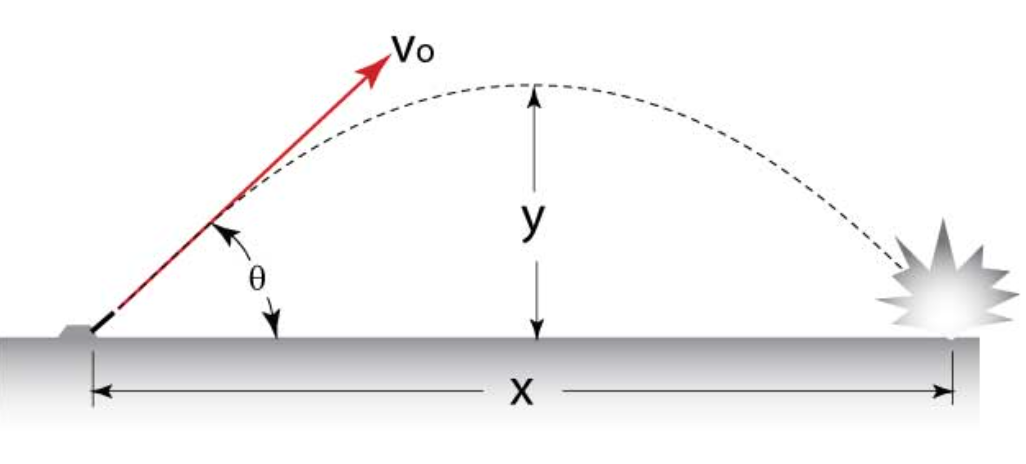
\includegraphics[width=0.8\textwidth]{Images/Kapittel2:Kinematikk/Prosjektile bevegelse 2.png}
    \caption{Prosjektilbevegelse}
    \label{fig:prosjektilbevegelse}
    \end{figure}

\exm{Ball som faller fra en klippe}{
En ball faller ut fra en klippe som er \(0.8 \, \text{m}\) høy og lander \(0.85 \, \text{m}\) unna foten av klippen. Vi skal beregne:
\begin{itemize}
    \item a) Startfarten \(v_0\)
    \item b) Sluttfarten \(v_1\), som er hastigheten rett før ballen treffer bakken.
\end{itemize}

\textbf{Del a: Beregn startfarten} \\

\textit{Metode:}
Vi bruker først posisjonslikningen i y-retning for å finne tiden \(t\) det tar før ballen treffer bakken. Siden ballen faller vertikalt uten startfart i y-retning (\(v_{0y} = 0\)), er posisjonslikningen i y-retning:
\[
y = y_0 + v_{0y} t + \frac{1}{2} a_y t^2.
\]
Vi vet at sluttposisjonen \(y = 0\), startposisjonen \(y_0 = 0.8 \, \text{m}\), og akselerasjonen \(a_y = -9.81 \, \text{m/s}^2\). Dette gir:
\[
0 = 0.8 + 0 \cdot t - \frac{1}{2} \cdot 9.81 \cdot t^2,
\]
som gir:
\[
t^2 = \frac{2 \cdot 0.8}{9.81},
\]
\[
\doubleunderline{t = \sqrt{\frac{1.6}{9.81}} \approx 0{,}4 \, \text{s}}
\]

Nå som vi har funnet tiden \(t = 0.4 \, \text{s}\), kan vi bruke posisjonslikningen i x-retning til å finne startfarten \(v_0\). Siden \(v_0 = v_{0x}\) og \(v_{0y} = 0\), er likningen i x-retning:
\[
x = v_{0x} t + \frac{1}{2} a_x t^2.
\]
Siden akselerasjonen i x-retning \(a_x = 0\), forenkles likningen til:
\[
x = v_{0x} t.
\]
Vi setter inn \(x = 0.85 \, \text{m}\) og \(t = 0.4 \, \text{s}\):
\[
0.85 = v_{0x} \cdot 0.4.
\]
Løs for \(v_{0x}\):
\[
\doubleunderline{v_0 = v_{0x} = \frac{0{,}85}{0{,}4} \approx 2{,}125 \, \text{m/s}}
\]

\textbf{Del b: Beregn sluttfarten rett før ballen treffer bakken} \\

\textit{Metode:}
For å finne sluttfarten \(v_1\) rett før ballen treffer bakken, må vi beregne både hastigheten i x- og y-retning ved \(t = 0.4 \, \text{s}\). Siden akselerasjonen i x-retning er null, forblir hastigheten i x-retning uendret:
\[
v_{1x} = v_{0x} = 2.125 \, \text{m/s}.
\]
For y-retningen bruker vi hastighetslikningen i y-retning:
\[
v_{1y} = v_{0y} + a_y t.
\]
Siden \(v_{0y} = 0\) og \(a_y = -9.81 \, \text{m/s}^2\), får vi:
\[
v_{1y} = 0 + (-9.81) \cdot 0.4 \approx -3.924 \, \text{m/s}.
\]

Den totale hastigheten \(v_1\) rett før ballen treffer bakken er summen av komponentene i x- og y-retning, og kan finnes ved Pythagoras' setning:
\[
v_1 = \sqrt{v_{1x}^2 + v_{1y}^2} = \sqrt{(2.125)^2 + (-3.924)^2} \approx \sqrt{4.515 + 15.4} \approx \sqrt{19.915} \approx 4.46 \, \text{m/s}.
\]

Dermed er sluttfarten rett før ballen treffer bakken \(\doubleunderline{v_1 \approx 4.46 \, \text{m/s}}\).
}

   \begin{figure}[ht!]
    \centering
    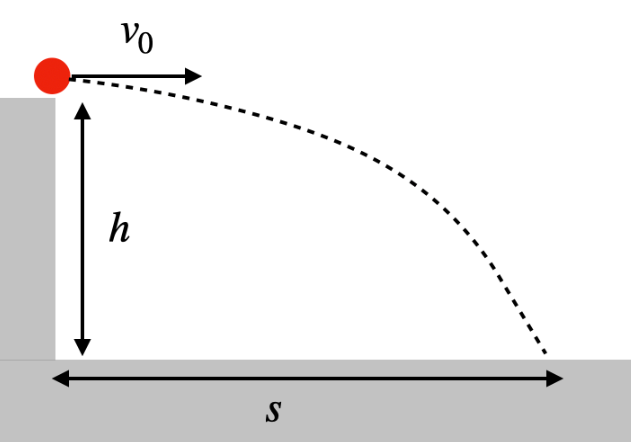
\includegraphics[width=0.8\textwidth]{Images/Kapittel2:Kinematikk/Ball ut av klippe.png}
    \caption{Ballen rett før den faller ut av klippen}
    \label{fig:Ball i klippen}
    \end{figure}

\oppgave{Prosjektilbevegelse}{%
En ball kastes horisontalt fra en klippe $h = 5\,\textrm{m}$ over bakken med startfart $v_0 = 10\,\textrm{m/s}$. Bruk $g = 9.81\,\textrm{m/s}^2$.
\begin{enumerate}[a)]
    \item Finn tiden ballen bruker på å treffe bakken.
    \item Finn den horisontale avstanden fra klippen til der ballen lander.
    \item Finn farten (størrelsen av hastighetsvektoren) rett før ballen treffer bakken.
\end{enumerate}
}

\newpage

\section{Sirkelbevegelse}

\textit{Sirkelbevegelse} oppstår når et objekt beveger seg i en bane som danner en sirkel. For eksempel, når en bil kjører rundt i en sving, eller når en stein knyttet til en tråd svinges rundt. Selv om farten (størrelsen på hastigheten) kan være den samme hele tiden, endres retningen til objektet hele tiden, siden det alltid svinger i en sirkel. For å få til denne bevegelsen må det virke en kraft som trekker objektet innover mot sentrum av sirkelen. Denne kraften fører til en akselerasjon som kalles \textit{sentripetalakselerasjon}.

\defn{Sentripetalakselerasjon}{
    Matematisk kan sentripetalakselerasjonen uttrykkes som:
    \begin{align}
        a_\perp = \frac{v^2}{r}
    \end{align}
    hvor \( a \) er akselerasjonen som virker innover mot sentrum av sirkelen, \( v \) er konstant banehastighet til objektet langs sirkelen (tangentiell hastighet), og \( r \) er radiusen til sirkelen. Denne formelen beskriver akselerasjonen som er nødvendig for å holde et objekt i jevn sirkelbevegelse.
}

Sentripetalakselerasjonen peker alltid mot sentrum av sirkelen, selv om objektet hele tiden beveger seg langs kanten av sirkelen. Dette er en viktig idé å forstå når vi ser på bevegelse i sirkulære baner.

\begin{figure}[ht!]
    \centering
    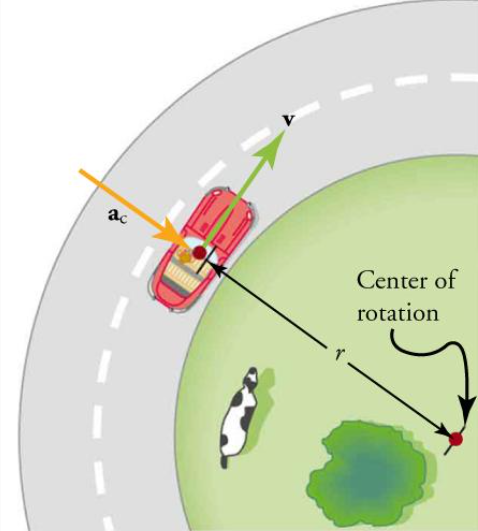
\includegraphics[width=0.4\textwidth]{Images/Kapittel2:Kinematikk/Sentripetal1.png}
    \caption{Bil svinger med sentripetalakselerasjon}
    \label{fig:Sentripetal2}
    \end{figure}


\defn{Utledning av sentripetalakselerasjon}{

    For et objekt som beveger seg i sirkel, endres retningen på hastighetsvektoren \( \vec{v} \), selv om størrelsen på \( v \) forblir konstant. Ser vi på to tidspunkt hvor hastigheten endrer seg fra \( \vec{v}_1 \) til \( \vec{v}_2 \), kan vi bruke forholdet mellom de formlike trekantene for \( \Delta \vec{v} \) og \( \Delta \vec{r} \), som gir oss:
    \[
    \frac{\Delta v}{v} = \frac{\Delta r}{r}.
    \]
    Der \( r \) er radiusen til sirkelen, og \( \Delta r \) er avstanden objektet har beveget seg langs sirkelen i løpet av et lite tidsintervall \( \Delta t \). 

  \[
    \frac{\Delta v}{\Delta t} = \frac{\Delta r \cdot v}{\Delta t \cdot r}
    \]

Vi lar \( \Delta t \to 0 \). Da vil \( \Delta r \to \Delta s \), så kan vi finne akselerasjonen ved å bruke grenseverdien når 

    \[
    a_\perp = \lim_{\Delta t \to 0} \frac{\Delta v}{\Delta t} = \lim_{\Delta t \to 0} \frac{\Delta v}{\Delta t} = \frac{\Delta r \cdot v}{\Delta t \cdot r}={v}\cdot \frac{v}{r}=\frac{v^2}{r}
    \]

    Dette er formelen for sentripetalakselerasjon, som alltid peker mot sentrum av sirkelen og sørger for at objektet holdes i sirkelbanen.
}

 \begin{figure}[ht!]
    \centering
    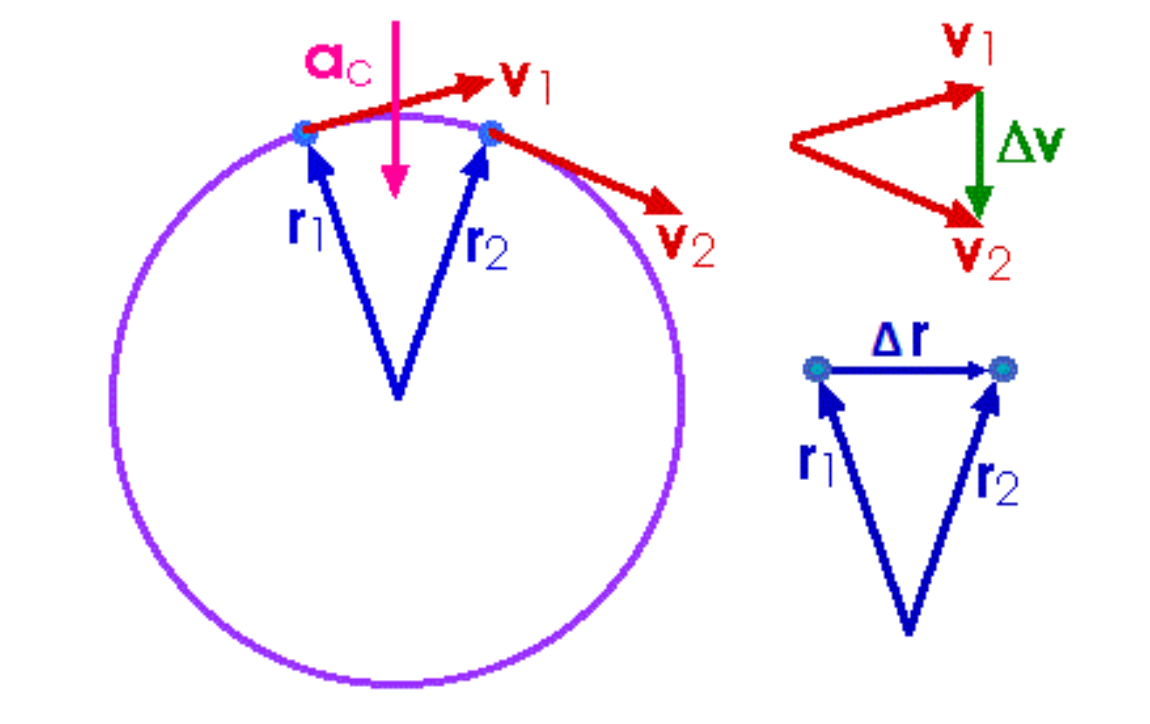
\includegraphics[width=0.7\textwidth]{Images/Kapittel2:Kinematikk/Sentripetalakselerasjon.png}
    \caption{Utledning av sentripetalakselerasjon}
    \label{fig:Sentripetalakselerasjon}
    \end{figure}
    
\newpage

\subsection{Omløpstid}

\textit{Omløpstid}, ofte kalt periodetid, refererer til den tiden det tar for et objekt å fullføre én fullstendig runde rundt en sirkel. Dette gjelder for objekter som beveger seg i sirkulære baner, som planeter rundt solen eller en satellitt i bane rundt jorden. Omløpstiden, vanligvis symbolisert som
\( T \), avhenger både av objektets hastighet og radiusen til sirkelen.

Omløpstiden er nært knyttet til sentripetalakselerasjonen, som holder objektet i sirkulær bevegelse. Selv om objektet har konstant fart, vil det oppleve akselerasjon fordi hastighetsretningen hele tiden endres. Jo kortere omløpstid, desto raskere må objektet bevege seg langs sirkelen, noe som fører til en høyere sentripetalakselerasjon.


\defn{Sentripetalakselerasjon ved omløpstid}{
    For et objekt som beveger seg i en sirkel med radius \( r \), kan sentripetalakselerasjonen uttrykkes som:
    \begin{align}
        a_\perp = \frac{4\pi^2 r}{T^2}.
    \end{align}
    Her er \( r \) radiusen til sirkelen, og \( T \) er omløpstiden. Denne formelen viser at akselerasjonen er omvendt proporsjonal med kvadratet av omløpstiden.
}

\tips{Viktige forhold ved sentripetalakselerasjon}{
    Husk at sentripetalakselerasjonen \( a_\perp \) kan uttrykkes på to måter:
    \[
    a_\perp = \frac{v^2}{r} = \frac{4 \pi^2 r}{T^2}.
    \]
    Dette viser at akselerasjonen er proporsjonal med kvadratet av hastigheten \( v \) og omvendt proporsjonal med kvadratet av omløpstiden \( T \). Dette er et av de viktigste forholdene å huske på når du jobber med sirkulær bevegelse.
}

\oppgave{Sirkelbevegelse og omløpstid}{%
Månens gjennomsnittlige avstand fra jorda er $r = 3.84 \cdot 10^8\,\textrm{m}$, og omløpstiden er $T = 27.3\,\textrm{dager}$.
\begin{enumerate}[a)]
    \item Gjør om omløpstiden til sekunder.
    \item Finn sentripetalakselerasjonen månen opplever ved hjelp av formelen $a_\perp = 4\pi^2 r / T^2$.
    \item Beregn månens banehastighet $v = 2\pi r / T$ og verifiser svaret ved å bruke $a_\perp = v^2/r$.
\end{enumerate}
}
